\documentclass[10pt,twoside]{scrreprt}
\usepackage{scrhack}
\renewcommand{\textfraction}{0.001}
\renewcommand{\topfraction}{0.999}   
\renewcommand{\bottomfraction}{0.999}

\usepackage{graphicx}
\usepackage{amsmath}
\usepackage{amssymb}
\usepackage[bibencoding=utf8, backend=biber, style=apa, minbibnames=1, maxnames=5]{biblatex}

\usepackage{a4,color}
\usepackage{tikz}

\usepackage{caption}
\usepackage{float}


\usepackage[T1]{fontenc}
\usepackage[utf8]{inputenc}



\definecolor{red}{rgb}{1,0,0}
\definecolor{green}{rgb}{0,1,0}
\definecolor{blue}{rgb}{0,0,1}
\definecolor{darkblue}{rgb}{0,0,0.8}

\definecolor{yellow}{rgb}{1,1,0}
\definecolor{lightblue}{rgb}{0,1,1}
\definecolor{magenta}{rgb}{1,0,1}
\definecolor{lightgrey}{rgb}{0.5,0.5,0.5}
\definecolor{grey}{rgb}{0.35,0.35,0.35}
\definecolor{darkgrey}{rgb}{0.2,0.2,0.2}
\definecolor{ockerrot}{rgb}{0.859,0.375,0.152}


\captionsetup{margin=0pt,font=small,labelfont=sc,labelformat=simple,format=plain,indention=3mm,
 labelsep=endash,textfont=sf,font=sf,singlelinecheck=false,figurename=Fig.,tablename=Tab.}


\fontfamily{ppl}\selectfont


\begin{document}

\chapter*{Abstract}
\addcontentsline{toc}{chapter}{Abstract}
Abstract stuff
	

\chapter{Introduction}
\section{LHC - Large Hadron Collider} % (fold)
\label{sec:lhc_large_hadron_collider}

The Large Hadron Collider (LHC) is the world's largest particle collider ever built. 

% section lhc_large_hadron_collider (end)

\chapter{Theory}

\section{RICH Detector} % (fold)
\label{sec:rich_detector}

Particle identification is a fundamental requirement at the LHCb experiment. Meaningful CP-violation measurements are only possible if hadron identification is available hence the ability to distinguish between kaons and pions is  essential.
% section rich_detector (end)

\section{Cherenkov-Radiation} % (fold)
\label{sec:cherenkov_radiation}

The speed of light in vacuum, \( \mathbf{c} \), is a universal physical constant. According to Einstein's special theory of relativity, \( c \) is the maximum speed at which all matter (or information) in the universe can travel. The speed at which light propagates in a medium, however, can be significantly less can \( c \).

Cherenkov radiation results when a charged particle travels through a dielectric medium with a speed greather than the speed of light through said medium. Moreover, the velocity that must be exceeded is the phase velocity \( v_p \) and not the group velocity \( v_G = \frac{\partial \omega}{\partial k} \).

\[ v_P = \frac{\lambda}{T} \quad \text{or} \quad \frac{\omega}{k}\]

As a charged particle travels through the medium, it disrupts the local electromagnetic field. If the particle travels slowly then the disturbance elastically relaxes to the mechinal equilibrium as the particle passes. However, if the particle travels fast enough, the limited response speed of the medium means that a disturbance is left in the wake of the particle, and the energy in this disturbance radiates as coherent shockwave.

\begin{figure}[htbp]
	\centering
		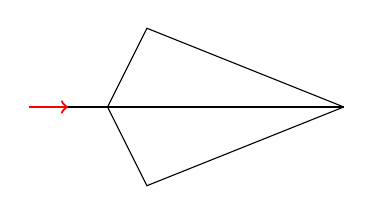
\begin{tikzpicture}
			\draw (-1,0) -- (3,0);
			\draw (0,0) -- (0.5,1) -- (3,0);
			\draw (0,0) -- (0.5,-1) -- (3,0);
			\draw[->, red, thick] (-1,0) -- (-0.5,0);
		\end{tikzpicture}
	\caption{Cherenkov radiation}
	\label{fig:label}
\end{figure}

\begin{align}
    x_p &= v_{p}\cdot t = \beta c t \nonumber \\
    x_{\text{em}} &= v_{\text{em}}\cdot t=\frac{c}{n}t \nonumber \\
    \cos\theta &= \frac{x_{\text{p}}}{x_{\text{em}}} = \frac{\frac{c}{n}t}{\beta c t} = \frac{1}{n\beta}
\end{align}

% section cherenkov_radiation (end)
\chapter{Methods}

\section{Hough Transform} % (fold)
\label{sec:hough_transform}

% section hough_transform (end)

\subsection{1D: Known Center - Find Radius} % (fold)
\label{sub:1d_known_center_find_radius}



% subsection 1d_known_center_find_radius (end)
\subsection{2D: Known Radius - Find Center} % (fold)
\label{sub:2d_known_radius_find_center}

% section 2d_known_radius_find_center (end)

\subsection{3D: Nothing is Known - Find Everything} % (fold)
\label{sub:3d_nothing_is_known_find_everything}

% subsection 3d_nothing_is_known_find_everything (end)

\section{Combinatorial approach}

The combinatorial approach relies on the fact that a circle is uniquely defined by 3 points. With 2 arbotrary points we couldn't tell which side the circle is
going to go. A third point gives us all the information we need. The general idea then is the following:

\begin{enumerate}
\item Build all possible triples of points given the data points
\item For all the point triples calculate the center and the radius of the potential circle
\item Due to constraints in the radius we can drop many of the circles with a radius bigger than a certain threshold
\item Create a histogram with the radius distribution. Peaks in the radius distribution hint to a circle.
\item We scan the radius histogram for peaks and look at the center point histogram for the given radius of a peak. If we have also a peak in the center point histogram
      the set of the points of the triples lie on a circle with a radius and center given by the histogram peaks.
\end{enumerate}

\subsection{Drawback}
	

There are 2 problems with this method.

\begin{itemize}
\item The combinatorics blow up with a high number of data points \( \binom{N}{3} \)
\item Also assuming we have a infinite amount of data points then we would also find an infinite number of circles
\end{itemize}

\chapter{Results}
\end{document}